\documentclass[12pt,notitlepage]{article}
\usepackage[bitstream-charter]{mathdesign}
\usepackage{inconsolata}
\usepackage[T1]{fontenc}
\usepackage{microtype}
\usepackage[utf8x]{inputenc}
\usepackage[letterpaper,margin=1in]{geometry}
\usepackage{titlesec}
\usepackage{graphicx}
\usepackage{wrapfig}
\usepackage{caption}
\usepackage{subcaption}
\usepackage{hyperref}
\usepackage{multicol}
\usepackage{booktabs}
\usepackage{tabu}

\newcommand\footnoteref[1]{\footnote{\url{#1}}}
\newcommand\tmts[0]{\texttt{tell me to survive}}

\titleformat{\section}{\normalfont\large}{\thesection}{0.5em}{}
\titleformat{\subsection}{\bfseries}{\thesubsection}{0.5em}{}
\titleformat{\subsubsection}{\normalfont}{\thesubsubsection}{0.5em}{}
\titlespacing*{\section}{0em}{0.75em}{0.3em}

\begin{document}
\begingroup
  \centering
  {\Large \texttt{tell me to survive}: Concreteness Fading and Visual
    Programming in Teaching Object-Oriented Programming\\[1em]}

  Andrew Jiang, Michael Mauer, and David Li\par
\endgroup

\section{Introduction and Motivation}

Much effort has gone towards methods to teach programming as an
overall concept, with systems like Scratch and CodeSpells
demonstrating how visual programming can successfully introduce
students to this field. Our goal is to teach the more specific topic
of object-oriented programming to novice programmers using these same
techniques, focusing on how to abstract and represent ideas such as
method definitions, subclassing, and overriding. Additionally, to
reinforce these concepts to an audience already somewhat familiar with
programming, we will introduce concreteness fading, transitioning
students from visual programming to directly writing code. This will
facilitate the learning of these specific higher-level concepts and
abstractions within computer science, which is important to
effectively educate and train the next generation of computer science
and software development students.

\section{Related Work}

The idea of visual programming manipulating robots or other objects in
a virtual world is not new; we list several games and projects in the
same vein, with some comparison to our project.

\begin{multicols}{2}
\begin{itemize}
\item CodeSpells\footnoteref{https://codespells.org/}
\item Scratch\footnoteref{https://scratch.mit.edu/}/Alice\footnoteref{http://www.alice.org/}
\item Looking Glass\footnoteref{https://lookingglass.wustl.edu/}
\item Hour of Code\footnoteref{https://code.org/learn}
\item LightBot\footnoteref{https://lightbot.com/hocflash.html}
\item Human Resource Machine\footnoteref{https://tomorrowcorporation.com/humanresourcemachine}
\item Blockly Games\footnoteref{https://blockly-games.appspot.com/}
\item BlockPy\footnoteref{https://github.com/RealTimeWeb/blockpy}
\end{itemize}
\end{multicols}

CodeSpells, Alice, Scratch, and Looking Glass are more free-form;
instead of specific puzzles or levels to solve, they simply place the
player in a sandbox. Looking Glass has metaphors for object-oriented
concepts, and covers more of them than our project does, but does not
employ concreteness fading. Hour of Code, LightBot, and Human Resource
Machine take the same puzzle-oriented approach our game does, but also
lack the concreteness fading aspect. Blockly Games is the most similar
to our approach, initially using blocks whose labels transition from
text descriptions to code, then changing to a text editor at the
end. However, it does not present a consistent game, changing the
theme and mechanics every few levels. BlockPy is more advanced,
enabling the player to seamlessly switch between code and visual
programming (and translating one to the other), but does not use
concreteness fading either.

\section{Methodology}

\tmts{} is a purely client-side, web-based game built on
HTML5/JavaScript using Python as its instructional language. The core
concept is manipulating robots in a game world via visual or
text-based programming in order to solve puzzles and accomplish
objectives.

\subsection{Concepts}

\begin{figure}[h]
  \centering
  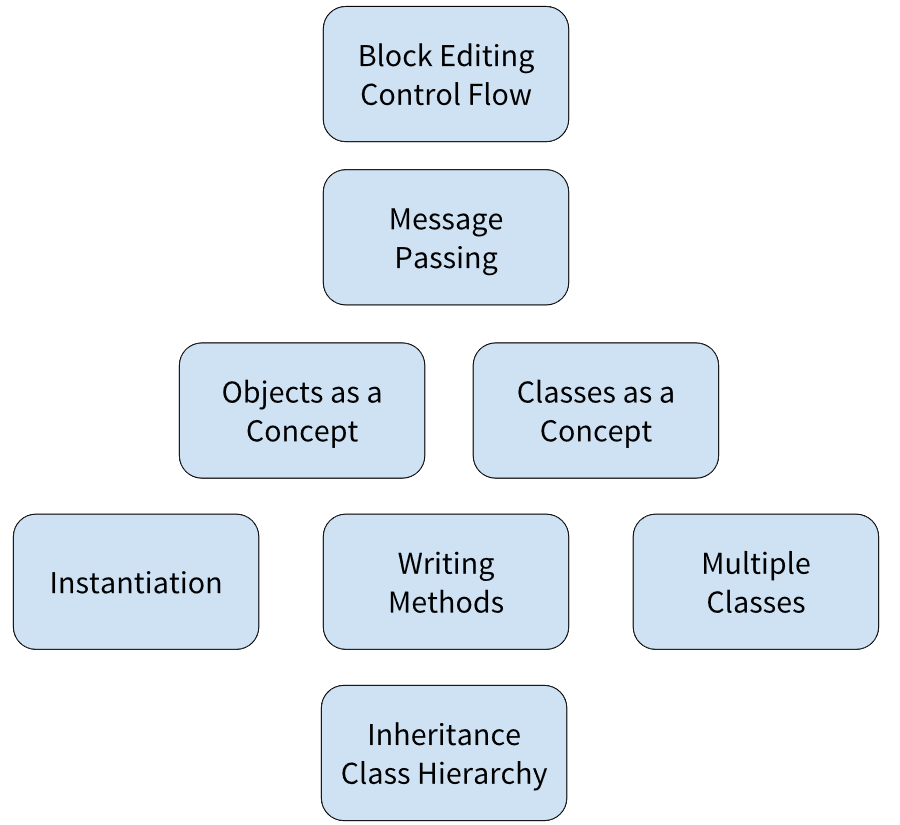
\includegraphics[width=.6\textwidth]{progression}
  \caption{Concept Progression}
\label{fig:progression}
\end{figure}

We limited our scope to the concepts in \autoref{fig:progression} in
order to limit the game length and complexity, and because of
implementation constraints. This means that advanced topics such as
abstract classes and polymorphism are not covered. This is an
acceptable trade-off because the purpose of this game is not to teach
OOP in its entirety, but rather to ease the conceptual transition for
new programmers.

\autoref{fig:progression} lists the progression of requisite skills up
to mastery of inheritance (our overall learning objective). Mastering
a skill in any given level in the diagram should require mastering
every skill in the previous level. For instance, using inheritance
effectively requires that the user is writing methods across several
classes in the hierarchy, then instantiating different types of objects
with those classes. These individual skills can then be further subdivided
down to the basics of using our click-and-drag block input system.

The level progression slowly moves concept by concept through the
skill tree, trying to introduce only one new concept per level;
otherwise, users are likely to get confused. For example, consider how
new robot types are introduced. At first the player must identify that
\texttt{MineRobot} (and other subclasses) can use functions for moving
and turning from the basic \texttt{Robot} class. Later on, there are
more complex relations, such as the way that \texttt{FrackingRobot}
overrides a function from \texttt{MineRobot}. Moreover, as new
concepts are introduced, old concepts are recombined to make new
puzzles. For example, the \texttt{HeavyLifter} is used in a context
such that it needs to use a function defined in the basic
\texttt{Robot} class. However, it also requires implementing that
method first.

\subsubsection{Concreteness Fading}

Our fading process has 3 stages. Initially, all blocks start off as
textual descriptions of what they do, e.g.\ ``tell \_ to \_'' for
method invocation or ``create a new \_ called \_'' for object
instantiation (see \autoref{fig:block-unfaded}). As the player
progresses, the labels on the blocks are faded into actual Python code,
as in \autoref{fig:block-faded}. Eventually, the player will be given
a text editor and asked to write the Python code themselves. Some
scaffolding always remains; for instance, the object hierarchy view always
remains accessible after it is introduced, and serves as a reference for
what classes and methods are available.

Beta testing found that changes to the blocks should not happen while
another concept is introduced, because otherwise, players are
overwhelmed by the number of new skills required. Thus, some levels
introduce no new object-oriented concepts, and instead, pose a simpler
puzzle focusing on usage of a newly faded block.

\begin{figure}[h]
\centering
\begin{subfigure}{.5\textwidth}
  \centering
  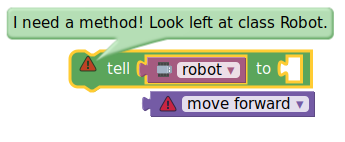
\includegraphics[width=.7\textwidth]{block_unfaded}
  \caption{An unfaded method invocation block.}\label{fig:block-unfaded}
\end{subfigure}%
\begin{subfigure}{.5\textwidth}
  \centering
  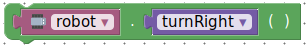
\includegraphics[width=.7\textwidth]{block_faded}
  \caption{The faded method invocation block.}\label{fig:block-faded}
\end{subfigure}
\label{fig:test}
\end{figure}


\subsection{Application Design}

Through user testing, we simplified our block interface as much as
possible. For instance, the repeat block was changed from accepting a
block subexpression to just a number. The player does not have access
to more complicated control flow such as branches and for loops. In
fact, even method invocation was simplified by ignoring parameters and
return values. Our goal was to focus more on a basic set of OOP
concepts and the corresponding syntax. Thus, we limited access to
features that would increase the complexity of solution code, while
ensuring that the player must use object-oriented concepts to solve
the level.

To further enforce object-oriented thinking, we imposed a block
limit. Similar to the way LightBot forces players to define functions
due to lack of space, we design levels such that there is no way to
finish within the block limit without defining a method. This forces
players to consider the class hierarchy and actually implement useful
methods they call on objects. Without this restriction, the hierarchy
(and thus our goal of teaching OOP) could potentially be disregarded.
% TODO: did we find a user that actually did that?

\subsection{Evaluation}

We evaluated the performance of the game by administering a pre-test
and post-test to all people who completed the game. Both tests were
entirely identical, 5 multiple-choice question quizzes testing both
object-oriented Python syntax and general concepts. Each question had
one correct answer, and a player's score can be any integer between
0 and 5 inclusive. The goal was to present questions that test for both
practical and more abstract understanding. The quizzes were strongly
integrated into the game itself, presented as an
``Robot Commander Aptitude Test'' and a ``Robot Commander Proficiency
Test''.

We targeted students who are currently enrolled in or have taken only
an introductory programming course. The game was advertised in CS 1110
(Spring 2016) at Cornell, and at Sparta High School, as well as
to specific students who have taken CS 1110 here. In general, we
looked for some procedural programming experience, with some or no
object-oriented experience (e.g.\ CS 1110 but not CS 2110).

\section{Results}

Our results are partially open data: all analysis scripts are under
the same license as the project itself (AGPLv3) and anonymized data is
available as well (random user IDs and completion time stats). This is
available in a separate repository,
\url{https://github.com/lidavidm/cs6360_analysis}.

\subsection{Pre- and Post-Test}

% reminder: update numbers
12 people completed the game and the post-test. The mean pre-test score
for those 12 people was 3.167 (s = 1.267). The mean post-test score was
4.25 (s = 0.754). We performed a paired t-test on the pre-test scores and
the post-test scores, and we found that the difference in means was
statistically significant, $t(11) = 3.767$, $p = 0.003$.

These results suggest that by playing the game, the players improved their
understanding of the concepts tested by the 5 questions, namely classes and
objects, method calls, initialization, inheritance, and overriding. Thus, we
can reasonably claim that the game is successful at teaching some of our
proposed learning objectives.

A potential confounding factor is that the correct answer to the second
test question can be inferred based on example code provided in later
questions. Specifically, the second question tests whether the player
understands the need for an object to be initialized and the required Python
syntax, but later questions show the player correct initialization code in
different contexts. In other words, learning of initialization and the related
syntax may have occurred during the pre-test and not while the game was being
played. The same could be said for question 3, which requires knowledge of
method call syntax; questions 4 and 5 display correct method call syntax in
question descriptions.

% Keep this paragraph?
One possible way to address the above problem is to form a control group.
The control group would take the pretest, do something unrelated for about
an hour (an anecdotal estimate of the time it takes a typical member of the
target audience to complete the game), and then take the posttest, which is
identical to the pretest. This would help us approximate the amount of
improvement that can attributed to the pre-test alone. Unfortunately, due to
time constraints and difficulty finding volunteers who fit the target audience
description, we were not able to include a control group in this study.

Another point to be wary of is when the pretest and posttest were completed.
Since the game was also distributed through the Internet and progress is
automatically saved in the browser cache, the pretest, game levels, and
posttest did not all have to completed in a single session. For example, one of
the players included in our analysis finished the posttest about five days
after they finished the pretest. In these cases, playing the game was not the
only activity that occurred between the completions of both tests, and those
other activities could have also contributed to learning.
% alternative: remove from analysis, along with other data points with long
% periods between pretest and posttest. might not affect the results significantly?

% discuss survivorship bias? and number of completed pretests?

\subsection{Subjective Impressions}

Our post-test also included four extra questions that were opinion-based.
Three of those consisted of asking the player how much they agreed with
the following three statements.

\begin{tabu}{Xlll}
\toprule
Statement & Mean score \\
\midrule
I enjoyed this game. & 1.08 \\
Before playing, I knew object-oriented programming. & 0.0 \\
After playing, I knew object-oriented programming better. & 1.25\\
\bottomrule
\\
\end{tabu}

The mean scores were obtained by mapping the five possible answers to integer
values as follows and computing the arithmetic mean normally:\\
\centerline{Strongly Agree → 2; Agree → 1; Neutral → 0; Disagree → -1; Strongly Disagree → -2}

These data are evidence that the game is relatively engaging and that players
perceived themselves getting better at object-oriented programming by playing
the game. On the other hand, these results may be partially due to the
Hawthorne effect.

The ninth and final question was free response and asked for any general
comments on the game. Overall, players responded positively. Not all left
feedback; many pointed out minor issues with usability and the interface,
such as the relatively slow animation speed, unclear directions, and lack
of examples.

We also evaluated some players in person.
One interesting behavior that we observed occurred when method definitions
faded from a block editor to a text editor. Some players who had trouble
recalling the exact syntax returned to the other methods that were still in
block-editor mode. They used the blocks, whose text had already faded into
python code, as references for the new method that they wanted to type. Given
that we did not tell the players about concreteness fading, this is perhaps
evidence that concreteness fading can be effectively applied to programming
games, and also that it was a good choice to make the fading as granular as
possible. However, players also said that they wished the interface allowed
them to more easily use the technique just discussed. Thus, a potential
improvement is to make example blocks or example code more accessible when
in the text-editor mode.

As for engagement statistics, we captured when each player started and
ended each level. This gives us a lower bound on the time spent to
complete a playthrough, as the end-of-level event was not always
recorded. The mean completion time was 7196 seconds, or almost exactly
two hours.

\subsection{TODO}

\section{Conclusions}

\end{document}
